% Made up for the tikra benchmark.
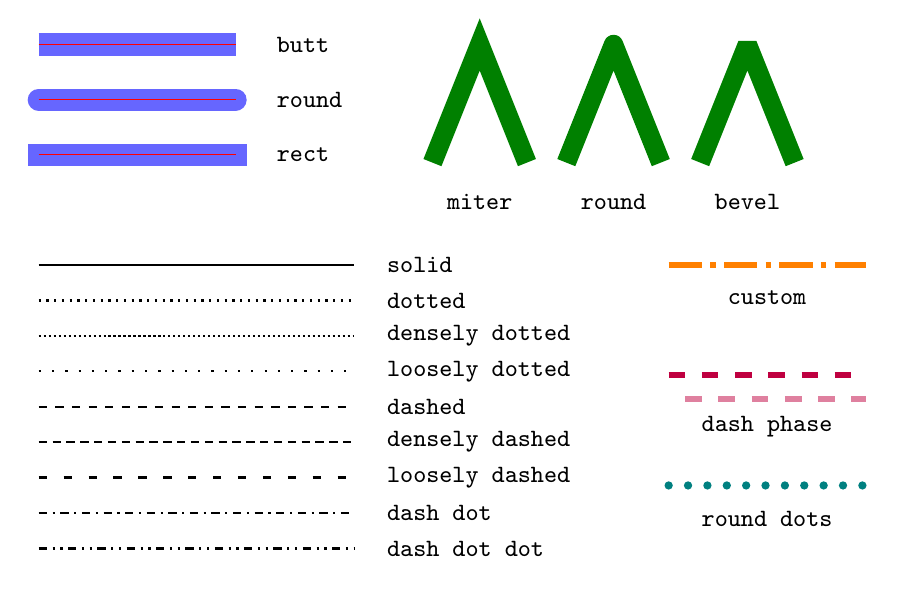
\begin{tikzpicture}[font=\small\ttfamily]
  % caps: the thin red line shows where each path really ends
  \foreach \c [count=\i from 0] in {butt, round, rect} {
    \draw[line width=8pt, line cap=\c, blue!60] (0,-\i*0.7) -- (2.5,-\i*0.7);
    \draw[red] (0,-\i*0.7) -- (2.5,-\i*0.7);
    \node[anchor=west] at (2.9,-\i*0.7) {\c};
  }
  % joins
  \foreach \j [count=\i from 0] in {miter, round, bevel} {
    \draw[line width=7pt, line join=\j, green!50!black] (5+\i*1.7,-1.5) -- (5.6+\i*1.7,0) -- (6.2+\i*1.7,-1.5);
    \node at (5.6+\i*1.7,-2) {\j};
  }
  % dash patterns
  \foreach \d [count=\i from 0] in {solid, dotted, densely dotted, loosely dotted, dashed,
      densely dashed, loosely dashed, dash dot, dash dot dot} {
    \draw[thick, \d] (0,-2.8-\i*0.45) -- (4,-2.8-\i*0.45);
    \node[anchor=west] at (4.3,-2.8-\i*0.45) {\d};
  }
  \draw[line width=2pt, orange, dash pattern=on 12pt off 3pt on 2pt off 3pt] (8,-2.8) -- (10.5,-2.8);
  \node[anchor=north] at (9.25,-3) {custom};
  \draw[line width=2pt, purple, dash pattern=on 6pt off 6pt] (8,-4.2) -- (10.5,-4.2);
  \draw[line width=2pt, purple!50, dash pattern=on 6pt off 6pt, dash phase=6pt] (8,-4.5) -- (10.5,-4.5);
  \node[anchor=north] at (9.25,-4.6) {dash phase};
  \draw[line width=3pt, teal, line cap=round, dash pattern=on 0pt off 7pt] (8,-5.6) -- (10.5,-5.6);
  \node[anchor=north] at (9.25,-5.8) {round dots};
\end{tikzpicture}
